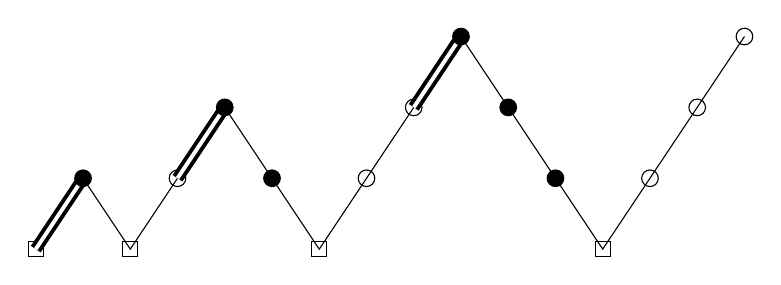
\begin{tikzpicture}[scale=1.2]
  \pgfmathsetmacro\hstep{0.5}
  \pgfmathsetmacro\vstep{0.75}
  \pgfmathsetmacro\ceps{0.08}   % size of square for coarse grid

% coarse solve only
  \draw     (-4*\hstep-\ceps,-\ceps) rectangle (-4*\hstep+\ceps,+\ceps);
  \draw[black,double,line width=0.5mm,double distance=0.5mm] (-4*\hstep,0.0) -- (-3*\hstep,\vstep);

% 2-level V-cycle
  \draw[black,thin] (-3*\hstep,\vstep) -- (-2*\hstep,0.0) -- (-\hstep,\vstep);
  \filldraw (-3*\hstep,\vstep) circle (2.5pt);
  \draw     (-2*\hstep-\ceps,-\ceps) rectangle (-2*\hstep+\ceps,+\ceps);
  \draw     (-\hstep,\vstep) circle (2.5pt);
  \draw[black,double,line width=0.5mm,double distance=0.5mm] (-\hstep,\vstep) -- (0.0,2*\vstep);

% 3-level V-cycle
  \draw[black,thin] (0.0,2*\vstep) -- (\hstep,\vstep) --  (2*\hstep,0.0) -- (3*\hstep,\vstep) -- (4*\hstep,2*\vstep);
  \filldraw (0.0,2*\vstep) circle (2.5pt);
  \filldraw (\hstep,\vstep) circle (2.5pt);
  \draw     (2*\hstep-\ceps,-\ceps) rectangle (2*\hstep+\ceps,+\ceps);
  \draw     (3*\hstep,\vstep) circle (2.5pt);
  \draw     (4*\hstep,2*\vstep) circle (2.5pt);
  \draw[black,double,line width=0.5mm,double distance=0.5mm] (4*\hstep,2*\vstep) -- (5*\hstep,3*\vstep);

% 4-level V-cycle
  \draw[black,thin] (5*\hstep,3*\vstep) -- (6*\hstep,2*\vstep) -- (7*\hstep,\vstep) --  (8*\hstep,0.0) -- (9*\hstep,\vstep) -- (10*\hstep,2*\vstep) -- (11*\hstep,3*\vstep);
  \filldraw (5*\hstep,3*\vstep) circle (2.5pt);
  \filldraw (6*\hstep,2*\vstep) circle (2.5pt);
  \filldraw (7*\hstep,\vstep) circle (2.5pt);
  \draw     (8*\hstep-\ceps,-\ceps) rectangle (8*\hstep+\ceps,+\ceps);
  \draw     (9*\hstep,\vstep) circle (2.5pt);
  \draw     (10*\hstep,2*\vstep) circle (2.5pt);
  \draw     (11*\hstep,3*\vstep) circle (2.5pt);

\end{tikzpicture}
